\section{Modelo del comportamiento}
  El sistema se encuentra organizado en un m\'odulo en el cual se destacan 3 acciones principales como se muestra en la figura 3:
  \begin{enumerate}
   \item Calcular ruta.
   \item Administrar Itinerario.
   \item Cambiar el idioma
  \end{enumerate}
  \begin{figure}[h]
      \centering
      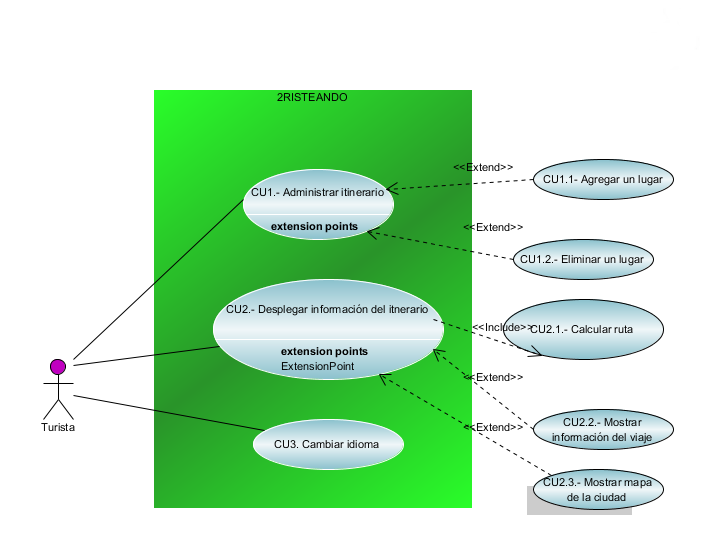
\includegraphics[width=12cm,height=10cm]{Imagenes/CasosUso/CU.png}
      \caption{Diagrama de casos de uso} 
      \label{fig:CU}
  \end{figure}
  
   \subsection{Actores del sistema}
    \subsubsection{Modelado de Actores}
    En esta secci\'on se describen las actividades que el Usuario podr\'a realizar.
    La figura siguiente muestra el perfil del Usuario que tendr\'a el sistema.
    
      \begin{figure}[h]
	\centering
	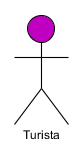
\includegraphics[width=2cm,height=3cm]{Imagenes/CasosUso/ActorTurista.PNG}
	\caption{Diagrama de actores del sistema}
	\label{fig:actores}
      \end{figure}
      
      
    \textbf{Nombre:} Turista
    \\
    \\
    \textbf{Descripci\'on:} El turista es la persona ingresar\'a al sistema para buscar un lugar de su interes en la zona centro del D.F. 
    Pede elegir entre 3 diferentes idiomas ingl\'es, frances y espa\~nol. Elegir\'a entre el itinerario generado por el sistema
    o personalizar\'a el suyo. Finalmente podr\'a evaluar el calculo del presupuesto ofrecido por el sistema.
    \\
    \\
    \textbf{Cantidad:} Uno por dispositivo m\'ovil.
    
 \subsection{Casos de Uso}
  En esta secci\'on se describen los casos de uso de la figura ~\ref{fig:CU}. De cada uno se detallar\'an los siguientes elementos:
  \begin{itemize}
   \item \textbf{Resumen:} Decripci\'on textual del caso de uso.
   \item \textbf{Actores:} Lista de actores que intervienen en el caso de uso.
   \item \textbf{Porp\'osito:} Una breve descripci\'on del objetivo que busca el actor al ejecutar el caso de uso.
   \item \textbf{Entradas:} Lista de datos de entrada requeridos durante la ejecuci\'on del caso de uso.
   \item \textbf{Salidas:} Lista de los datos de salida que otorga el sistema durante la ejecuci\'on del caso de uso.
   \item \textbf{Precondiciones:} Descripci\'on de las operaciones o condiciones que se deben cumplir para
   que el caso de uso pueda ejecutarse correctamente.
   \item \textbf{Postcondiciones:} Lista de los cambios que ocurrir\'an en el sistema despu\'es de la ejecuci\'on
   del caso de uso.
   \item \textbf{Errores:} Lista de los posibles errores que pueden surgir durante la ejecuci\'on del caso de uso.
   \item \textbf{Trayectorias:} Secuencia de pasos que ejecutar\'a el caso de uso.
  \end{itemize}



